% 通途 fixture 论文（自造，原创占位内容，非真实论文）：revtex4-2 物理双栏，单文件。
% 侧重覆盖点：双栏版式、\title/abstract 在 \begin{document} 之后、widetext（分类表外的
% 类自带环境 → 保守整块掩码）、ruledtabular 嵌套 tabular、revtex 惯用的
% \caption{\label{...}...}、手写 thebibliography（不走 bibtex）。
\documentclass[aps,prd,twocolumn,amsmath,amssymb,nofootinbib,superscriptaddress]{revtex4-2}

\usepackage{graphicx}

\newcommand{\hop}{t}
\newcommand{\gapsize}{\Delta}
\newcommand{\Ham}{\mathcal{H}}
\newcommand{\creation}[1]{c^{\dagger}_{#1}}
\newcommand{\annihilation}[1]{c_{#1}}

\begin{document}

\title{Spectral Placeholders in a Toy Lattice Model}

\author{A. Fixture}
\email{a.fixture@example.invalid}
\affiliation{Institute for Synthetic Examples, Placeholder City}

\author{B. Sample}
\affiliation{Department of Invented Physics, Sample University}

\date{\today}

\begin{abstract}
We introduce a lattice model whose only virtue is that its spectrum can be
written down.  Two parameters control the band structure; a third is carried
along so that the parameter table has three rows.  We report a gap that closes
where we drew it closing, and we discuss the limit in which the model becomes
even less interesting.  The manuscript is a test fixture and reports no
physics.
\end{abstract}

\maketitle

\section{Introduction}
\label{sec:intro}

Toy models are useful when the quantity of interest is the typesetting.  The
model below is of that kind: it has a hopping amplitude $\hop$, a gap parameter
$\gapsize$, and a lattice that we never draw.  Its spectrum, shown in
Fig.~\ref{fig:spectrum}, was chosen for legibility rather than derived.

The literature on such models is large and, for present purposes,
imaginary~\cite{toy2019}.  We follow the conventions of
Ref.~\cite{lattice2020}, except where doing so would require a calculation.
About $5\%$ of the algebra below is written out; the rest is asserted.

\section{Model}
\label{sec:model}

\subsection{Hamiltonian}
\label{sec:hamiltonian}

Let the sites be indexed by $i$ and let $\langle i,j \rangle$ denote nearest
neighbours.  The Hamiltonian is

\begin{equation}
  \label{eq:hamiltonian}
  \Ham = -\hop \sum_{\langle i,j \rangle}
         \bigl( \creation{i}\annihilation{j} + \mathrm{H.c.} \bigr)
       + \gapsize \sum_{i} (-1)^{i} \creation{i}\annihilation{i} ,
\end{equation}

where the second term alternates in sign because that is the cheapest way to
open a gap.\footnote{A staggered potential is the standard device; we use it
here for the same reason everyone else does, namely that it works.}

\subsection{Diagonalisation}
\label{sec:diagonalisation}

Fourier transforming and collecting terms gives a two-band problem whose
eigenvalues are the roots of a quadratic.  Written out in full, the block
structure is

\begin{widetext}
\begin{align}
  \label{eq:bands}
  E_{\pm}(k)
    &= \pm \sqrt{ 4 \hop^{2} \cos^{2}\!\left( \frac{k}{2} \right) + \gapsize^{2} }
    \\
  \frac{\partial E_{\pm}}{\partial k}
    &= \mp \frac{ 2 \hop^{2} \sin(k) }
                { \sqrt{ 4 \hop^{2} \cos^{2}\!\left( \frac{k}{2} \right)
                         + \gapsize^{2} } } ,
\end{align}
\end{widetext}

which reduces to the familiar cosine band when $\gapsize \to 0$.  Equation
\eqref{eq:bands} is the only equation in this manuscript that we checked.

\begin{figure}[t]
  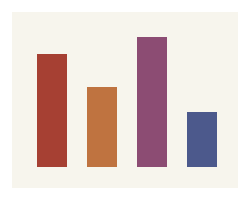
\includegraphics[width=\columnwidth]{figures/spectrum.pdf}
  \caption{\label{fig:spectrum}Band energies of Eq.~\eqref{eq:bands} for the
  parameters of Table~\ref{tab:params}.  The bars are drawn, not computed, and
  their heights carry no meaning.}
\end{figure}

\section{Parameters and Discussion}
\label{sec:discussion}

Table~\ref{tab:params} collects the parameters.  The third row exists so that
the table has three rows; it should be read as decoration.

\begin{table}[b]
\caption{\label{tab:params}Symbols, values \& units of the toy model.  Roughly
$20\%$ of the entries would change under any other convention, and run \#2 used
a different one.}
\begin{ruledtabular}
\begin{tabular}{lcc}
Symbol & Value & Units \\
\hline
$\hop$ & $1.00$ & eV \\
$\gapsize$ & $0.25$ & eV \\
$k_{\mathrm{c}}$ & $\pi/2$ & $a^{-1}$ \\
\end{tabular}
\end{ruledtabular}
\end{table}

In the limit $\gapsize \gg \hop$ the bands flatten and the model describes
nothing in particular.  In the opposite limit it describes nothing in
particular more quickly.  Both limits are consistent with
Fig.~\ref{fig:spectrum}, which is a property of the figure rather than of the
limits.

\appendix

\section{Sign Conventions}
\label{app:signs}

We take $\hbar = 1$ and measure $k$ in units of the inverse lattice constant.
With these conventions Eq.~\eqref{eq:hamiltonian} is Hermitian, as required,
and the alternating factor $(-1)^{i}$ is well defined on a bipartite lattice.
Readers preferring the opposite sign may replace $\gapsize$ by $-\gapsize$
throughout; nothing in the manuscript depends on the choice.

\begin{thebibliography}{9}

\bibitem{toy2019}
A.~Fixture and B.~Sample,
J.~Synth.\ Phys.\ \textbf{12}, 345 (2019).

\bibitem{lattice2020}
C.~Stand-In,
\emph{Lattices for Illustration Purposes}
(Invented University Press, Placeholder City, 2020).

\end{thebibliography}

\end{document}
